%%%%%%%%%%%%%%%%%%%%%%%%%%%%%%%%%%%%%%%%%
% Lachaise Assignment
% LaTeX Template
% Version 1.0 (26/6/2018)
%
% This template originates from:
% http://www.LaTeXTemplates.com
%
% Authors:
% Marion Lachaise & François Févotte
% Vel (vel@LaTeXTemplates.com)
%
% License:
% CC BY-NC-SA 3.0 (http://creativecommons.org/licenses/by-nc-sa/3.0/)
% 
%%%%%%%%%%%%%%%%%%%%%%%%%%%%%%%%%%%%%%%%%

%----------------------------------------------------------------------------------------
%	PACKAGES AND OTHER DOCUMENT CONFIGURATIONS
%----------------------------------------------------------------------------------------

\documentclass{article}

%%%%%%%%%%%%%%%%%%%%%%%%%%%%%%%%%%%%%%%%%
% Lachaise Assignment
% Structure Specification File
% Version 1.0 (26/6/2018)
%
% This template originates from:
% http://www.LaTeXTemplates.com
%
% Authors:
% Marion Lachaise & François Févotte
% Vel (vel@LaTeXTemplates.com)
%
% License:
% CC BY-NC-SA 3.0 (http://creativecommons.org/licenses/by-nc-sa/3.0/)
% 
%%%%%%%%%%%%%%%%%%%%%%%%%%%%%%%%%%%%%%%%%

%----------------------------------------------------------------------------------------
%	PACKAGES AND OTHER DOCUMENT CONFIGURATIONS
%----------------------------------------------------------------------------------------

\usepackage{amsmath,amsfonts,stmaryrd,amssymb} % Math packages
\usepackage[dvipsnames]{xcolor}
\usepackage{enumerate} % Custom item numbers for enumerations
\usepackage{hyperref}
\usepackage[ruled,vlined]{algorithm2e} % Algorithms

\usepackage[framemethod=tikz]{mdframed} % Allows defining custom boxed/framed environments

\usepackage{listings} % Required for insertion of code

\newcommand{\randomcolor}{%
  \definecolor{randomcolor}{RGB}
   {
    \pdfuniformdeviate 256,
    \pdfuniformdeviate 256,
    \pdfuniformdeviate 256
   }%
  \color{randomcolor}%
}

\definecolor{codegreen}{rgb}{0,0.6,0}
\definecolor{codegray}{rgb}{0.5,0.5,0.5}
\definecolor{codepurple}{rgb}{0.58,0,0.82}
\definecolor{backcolour}{rgb}{1,1,1}
\lstdefinestyle{mystyle}{
    backgroundcolor=\color{backcolour},   
    commentstyle=\color{codegreen},
    keywordstyle=\color{magenta},
    numberstyle=\tiny\color{codegray},
    stringstyle=\color{codepurple},
    basicstyle=\ttfamily\footnotesize,
    breakatwhitespace=false,         
    breaklines=true,                 
    captionpos=b,                    
    keepspaces=true,                 
    numbers=left,                    
    numbersep=5pt,                  
    showspaces=false,                
    showstringspaces=false,
    showtabs=false,                  
    tabsize=2
}
\renewcommand{\lstlistingname}{Código}% Listing -> Algorithm
\lstset{style=mystyle}


%\usepackage{listings} % File listings, with syntax highlighting
%\lstset{
%	basicstyle=\ttfamily, % Typeset listings in monospace font
%}

%----------------------------------------------------------------------------------------
%	DOCUMENT MARGINS
%----------------------------------------------------------------------------------------

\usepackage{geometry} % Required for adjusting page dimensions and margins

\geometry{
	paper=a4paper, % Paper size, change to letterpaper for US letter size
	top=2.5cm, % Top margin
	bottom=3cm, % Bottom margin
	left=2.5cm, % Left margin
	right=2.5cm, % Right margin
	headheight=14pt, % Header height
	footskip=1.5cm, % Space from the bottom margin to the baseline of the footer
	headsep=1.2cm, % Space from the top margin to the baseline of the header
	%showframe, % Uncomment to show how the type block is set on the page
}

%----------------------------------------------------------------------------------------
%	FONTS
%----------------------------------------------------------------------------------------

\usepackage[utf8]{inputenc} % Required for inputting international characters
\usepackage[T1]{fontenc} % Output font encoding for international characters

\usepackage{XCharter} % Use the XCharter fonts
\usepackage{pgfplots}
\usepackage{multicol}
%----------------------------------------------------------------------------------------
%	COMMAND LINE ENVIRONMENT
%----------------------------------------------------------------------------------------

% Usage:
% \begin{commandline}
%	\begin{verbatim}
%		$ ls
%		
%		Applications	Desktop	...
%	\end{verbatim}
% \end{commandline}

\mdfdefinestyle{commandline}{
	leftmargin=10pt,
	rightmargin=10pt,
	innerleftmargin=15pt,
	middlelinecolor=black!50!white,
	middlelinewidth=2pt,
	frametitlerule=false,
	backgroundcolor=black!5!white,
	frametitle={Command Line},
	frametitlefont={\normalfont\sffamily\color{white}\hspace{-1em}},
	frametitlebackgroundcolor=black!50!white,
	nobreak,
}

% Define a custom environment for command-line snapshots
\newenvironment{commandline}{
	\medskip
	\begin{mdframed}[style=commandline]
}{
	\end{mdframed}
	\medskip
}

%----------------------------------------------------------------------------------------
%	FILE CONTENTS ENVIRONMENT
%----------------------------------------------------------------------------------------

% Usage:
% \begin{file}[optional filename, defaults to "File"]
%	File contents, for example, with a listings environment
% \end{file}

\mdfdefinestyle{file}{
	innertopmargin=1.6\baselineskip,
	innerbottommargin=0.8\baselineskip,
	topline=false, bottomline=false,
	leftline=false, rightline=false,
	leftmargin=2cm,
	rightmargin=2cm,
	singleextra={%
		\draw[fill=black!10!white](P)++(0,-1.2em)rectangle(P-|O);
		\node[anchor=north west]
		at(P-|O){\ttfamily\mdfilename};
		%
		\def\l{3em}
		\draw(O-|P)++(-\l,0)--++(\l,\l)--(P)--(P-|O)--(O)--cycle;
		\draw(O-|P)++(-\l,0)--++(0,\l)--++(\l,0);
	},
	nobreak,
}

% Define a custom environment for file contents
\newenvironment{file}[1][File]{ % Set the default filename to "File"
	\medskip
	\newcommand{\mdfilename}{#1}
	\begin{mdframed}[style=file]
}{
	\end{mdframed}
	\medskip
}

%----------------------------------------------------------------------------------------
%	NUMBERED QUESTIONS ENVIRONMENT
%----------------------------------------------------------------------------------------

% Usage:
% \begin{question}[optional title]
%	Question contents
% \end{question}

\mdfdefinestyle{question}{
	innertopmargin=1.2\baselineskip,
	innerbottommargin=0.8\baselineskip,
	roundcorner=5pt,
	nobreak,
	singleextra={%
		\draw(P-|O)node[xshift=1em,anchor=west,fill=white,draw,rounded corners=5pt]{%
		Pregunta \theQuestion\questionTitle};
	},
}

\newcounter{Question} % Stores the current question number that gets iterated with each new question

% Define a custom environment for numbered questions
\newenvironment{question}[1][\unskip]{
	\bigskip
	\stepcounter{Question}
	\newcommand{\questionTitle}{~#1}
	\begin{mdframed}[style=question]
}{
	\end{mdframed}
	\medskip
}

%----------------------------------------------------------------------------------------
%	WARNING TEXT ENVIRONMENT
%----------------------------------------------------------------------------------------

% Usage:
% \begin{warn}[optional title, defaults to "Warning:"]
%	Contents
% \end{warn}

\mdfdefinestyle{warning}{
	topline=false, bottomline=false,
	leftline=false, rightline=false,
	nobreak,
	singleextra={%
		\draw(P-|O)++(-0.5em,0)node(tmp1){};
		\draw(P-|O)++(0.5em,0)node(tmp2){};
		\fill[black,rotate around={45:(P-|O)}](tmp1)rectangle(tmp2);
		\node at(P-|O){\color{white}\scriptsize\bf !};
		\draw[very thick](P-|O)++(0,-1em)--(O);%--(O-|P);
	}
}

% Define a custom environment for warning text
\newenvironment{warn}[1][Warning:]{ % Set the default warning to "Warning:"
	\medskip
	\begin{mdframed}[style=warning]
		\noindent{\textbf{#1}}
}{
	\end{mdframed}
}

%----------------------------------------------------------------------------------------
%	INFORMATION ENVIRONMENT
%----------------------------------------------------------------------------------------

% Usage:
% \begin{info}[optional title, defaults to "Info:"]
% 	contents
% 	\end{info}

\mdfdefinestyle{info}{%
	topline=false, bottomline=false,
	leftline=false, rightline=false,
	nobreak,
	singleextra={%
		\fill[black](P-|O)circle[radius=0.4em];
		\node at(P-|O){\color{white}\scriptsize\bf i};
		\draw[very thick](P-|O)++(0,-0.8em)--(O);%--(O-|P);
	}
}

% Define a custom environment for information
\newenvironment{info}[1][Info:]{ % Set the default title to "Info:"
	\medskip
	\begin{mdframed}[style=info]
		\noindent{\textbf{#1}}
}{
	\end{mdframed}
}
 % Include the file specifying the document structure and custom commands

%----------------------------------------------------------------------------------------
%	ASSIGNMENT INFORMATION
%----------------------------------------------------------------------------------------

\title{ITC-ADA-C1-2023: Assignment \#4} % Title of the assignment

\author{Luis Ballado\\ \texttt{luis.ballado@cinvestav.mx}} % Author name and email address

\date{CINVESTAV UNIDAD TAMAULIPAS --- \today} % University, school and/or department name(s) and a date

%----------------------------------------------------------------------------------------

\begin{document}

\maketitle % Print the title

%----------------------------------------------------------------------------------------
%	INTRODUCTION
%----------------------------------------------------------------------------------------

%--- cambiar estilo de secciones
\titleformat{\section}  % which section command to format
  {\fontsize{12}{12}\bfseries} % format for whole line
  {\thesection} % how to show number
  {1em} % space between number and text
  {} % formatting for just the text
  [] % formatting for after the text

\section{Un grafo es bipartita si todos sus vértices pueden ser divididos en dos subconjuntos disjuntos X y Y de forma tal que cada arco conecte un vértice en X con uno en Y.}

\begin{question}
  \textbf{Diseñe e implemente un algoritmo basado en DFS para verificar si un grafo es bipartita.}
\end{question}
  
%se responde aquí
\textit{Visto en clase que la implementación de un algoritmo DFS en su versión recursiva no hace uso de una implementación de tipo stack, ya que hace uso del call to stack que la recursión está creando.\\Un algoritmo DFS con recursión puede quedar como a continuación:}

\begin{center}
  \begin{minipage}{0.7\linewidth} % Adjust the minipage width to accomodate for the length of algorithm lines
    \begin{algorithm}[H] 
      \SetKwInOut{Input}{entrada}\SetKwInOut{Output}{salida}
      \SetKwFunction{KwFn}{Fn}
      \SetAlgoLined
      \SetKwProg{Function}{Function}{}{end}
      \Input{$G$: Un grafo representado como lista de adyacencia}
      \Input{$nodo$: El nodo de inicio}
      \DontPrintSemicolon
      \caption{Algoritmo DFS version recursiva}
      \label{alg:loop}
      visitado $\leftarrow$ {falso};\\
      DFS(nodo);\\
      \Function{DFS(u):}{
        \If{visitado[u] = true}{
          return;
        }
        print(u);\\
        visitado[u] $\leftarrow$ true;\\
        \For{v $\in$ G[u].vecinos()}{
          DFS(v);
        }
      }
    \end{algorithm}
  \end{minipage}
\end{center}

Recordando que un grafo es bipartita sí y sólo sí, éste puede ser dividido en dos conjuntos U \& V tales que no existe una arista entre ambos.\\

Para saber si hablamos de un grafo bipartita podemos comenzar en cualquier nodo, marcarlo como visitado.\\

Basandonos en ello buscaremos tomar la idea de exploración DFS para un grafo dado en texto.txt encontrar si éste es bipartito o no, proponemos el siguiente pseudo-código:


\begin{center}
  \begin{minipage}{0.7\linewidth} % Adjust the minipage width to accomodate for the length of algorithm lines
    \begin{algorithm}[H] 
      \SetKwInOut{Input}{entrada}\SetKwInOut{Output}{salida}
      \SetKwFunction{KwFn}{Fn}
      \SetAlgoLined
      \SetKwProg{Function}{Function}{}{end}
      \Input{$G$: Un grafo representado como lista de adyacencia}
      \DontPrintSemicolon
      \caption{Algoritmo DFS Bipartita}
      \label{alg:loop}

      \Function{DFS(vertice,vector\_visitado,lista\_adyacencia(G)):}{
        marcar vertice como visitado en vector\_visitado\\

        \For{v $\in$ G[vertice]}{
          \If{v no ha sido visitado}{
            marcar v como visitado siempre y cuando el vertice fue visitado\\
            \If{DFS(v,vector\_visitado,lista\_adyacencia) == false}{
              return false\\
            }
          }\ElseIf{visitado[v] == visitado[vector]}{
            return false\\
          }
        }
        return true\\
      }
      
      vector\_visitado de la cardinalidad del núm de aristas\\
      \For{v $\in$ G[u].vecinos()}{
        \If{v no ha sido visitado}{
          marcar v como visitado\\
          \If{DFS(v,vector\_visitado,lista\_adyacencia) == false}{
            bipartita = false\\
            break\\
          }
        }
      }

      print(bipartita)
      
    \end{algorithm}
  \end{minipage}
\end{center}


\subsection{Implementación y corridas}

\href{https://github.com/luisballado/ADA/blob/main/practice_code/tarea4_bipartito.cpp}{ver código en github}\\

Ejecutar desde una terminal

% Command-line "screenshot"
\begin{commandline}
\begin{verbatim}
  $ g++ tarea4_bipartito.cpp -o bip
  $ ./bip < grafo.txt
  El grafo de entrada no es bipartito.
\end{verbatim}
\end{commandline}

\newpage
\begin{question}
  \textbf{Analice matemáticamente la complejidad temporal de su algoritmo. Presente ejemplos de sus corridas.}
\end{question}

La complejidad temporal del algoritmo DFS que usa recursividad es O(|V| + |E|), donde |V| es el número de vértices en el gráfico, y |E| es el número de aristas.\\

En el peor de los casos, el algoritmo visita cada vértice y borde del gráfico exactamente una vez. Específicamente, cada vértice se agrega al conjunto visitado exactamente una vez y cada borde se explora exactamente una vez. El ciclo for que itera a través de los vecinos de cada vértice toma un tiempo O(grado(v)), donde grado(v) es el grado (es decir, el número de aristas que inciden en) el vértice v. Por lo tanto, la complejidad temporal total es O (|V| + |E|).\\

Tenga en cuenta que esta complejidad de tiempo supone que el gráfico se representa como una lista de adyacencia. Si el gráfico se representa como una matriz de adyacencia, la complejidad temporal de comprobar si existe una arista entre dos vértices requiere un tiempo O(1), por lo que la complejidad temporal total se convierte en $O(|V|^2)$.\\

\textbf{Ejemplos:}\\

Dado el siguiente grafo:

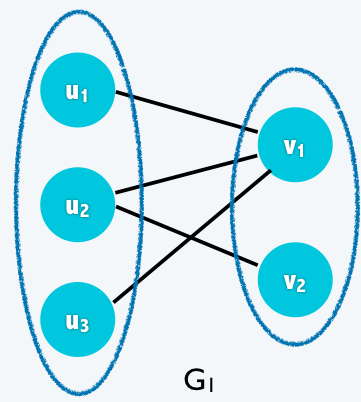
\includegraphics[scale=0.3]{bip.png}

se representa como un archivo de texto como:\\
5 4\\
0 1\\
1 2\\
1 4\\
2 3\\

\begin{commandline}
\begin{verbatim}
  $ cat grafo.txt
  5 4
  0 1
  1 2
  1 4
  2 3
  $ ./bip < grafo.txt
  El grafo de entrada es bipartito.
\end{verbatim}
\end{commandline}
\newpage
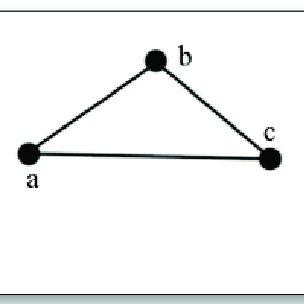
\includegraphics[scale=0.9]{nobip.jpg}

se representa como un archivo de texto como:\\
3 3\\
0 1\\
1 2\\
2 0\\

\begin{commandline}
\begin{verbatim}
  $ cat grafo.txt
  3 3
  0 1
  1 2
  2 0
  $ ./bip < grafo_1.txt
  El grafo de entrada no es bipartito.
\end{verbatim}
\end{commandline}

Se incluyen varios grafos ya representados como archivos de entrada:\\
núm vertices - num aristas\\
vertice origen - vertice destino\\
vertice origen - vertice destino\\
.. etc\\

\newpage
\section{Diseñe e implemente un algoritmo basado en DFS que permita resolver eficientemente el problema 3.8 de la pág 102 del libro de Dasgupta. Analice matemáticamente la complejidad temporal de su algoritmo}

3.8. Vaciando agua. Tenemos tres recipientes cuyos tamaños son de 10 lts, 7 lts y 4 lts, respectivamente.\\
Los recipientes de 7 lts y 4 lts comienzan llenos de agua, pero el recipiente de 10 lts está inicialmente vacío. Tenemos permitido un tipo de operación: verter el contenido de un recipiente en otro, deteniéndose sólo cuando el contenedor de origen está vacío o el contenedor de destino está lleno. Queremos saber si hay una secuencia de vertidos que deja exactamente 2 lts en el recipiente de 7 o 4 lts.

\begin{question}
  \textbf{Modele esto como un problema de grafos: proporcione una definición precisa del gráfico involucrado y plantee la pregunta específica sobre este grafo que necesita ser respondida.}\\
\end{question}

Para modelar este problema como un problema de grafos, podemos representar los posibles estados de los tres contenedores como nodos en un grafo, donde cada nodo representa una combinación particular de niveles de agua en los tres contenedores. Luego, podemos agregar bordes entre nodos para representar las operaciones de vertido, donde un borde del nodo A al nodo B representa el vertido de agua de un recipiente a otro, lo que da como resultado un nuevo estado representado por el nodo B. La pregunta específica que debe responderse es si existe una ruta desde un nodo de inicio hasta un nodo de destino que deja exactamente 2 pintas en el contenedor de 7 o 4 pintas.\\

Cada nodo representa una configuración particular de los contenedores, y un borde entre dos nodos representa una operación de vertido válida que se puede realizar para pasar de una configuración a la otra. En concreto, cada nodo del gráfico corresponde a una tupla de la forma (a, b, c) que representa la cantidad actual de agua en cada recipiente, y existe una arista entre los nodos (a, b, c) y (a', b', c') si y solo si es posible verter agua de un recipiente a otro para pasar de (a, b, c) a (a', b', c').\\

Podemos considerar partir de la condición inicial (0, 7, 4) y llegar a la solución bajo los siguientes pasos 7 pasos:
\begin{enumerate}
\item 0, \textbf{7}, \textbf{4} - INICIO --> Vaciar 4 litros del tanque3 al tanque1
\item 4, \textbf{7}, 0 - Vaciar 6 litros del tanque2 al tanque1
\item \textbf{10}, 1, 0 - Vaciar 4 litros del tanque1 al tanque3
\item 6, 1, \textbf{4} - Vaciar 4 litros del tanque3 al tanque2
\item \textbf{6}, 5, 0 - Vaciar 4 litros del tanque1 al tanque3
\item 2, 5, \textbf{4} - Vaciar 2 litros del tanque3 al tanque2
\item 2, 7, \textcolor{red}{2} - Tanque1 queda con 2 litros, Tanque2 queda con 7 litros y Tanque3 queda con 2 litros
\end{enumerate}

También existe una solución para llegar con 8 pasos:
\begin{enumerate}
\item 0, \textbf{7}, \textbf{4} - INICIO --> Vaciar 7 litros del tanque2 al tanque1
\item 7, 0, \textbf{4} - Vaciar 3 litros del tanque3 al tanque1
\item 10, 0, \textbf{1} - Vaciar 1 litro del tanque3 al tanque2
\item \textbf{10}, 1, 0 - Vaciar 4 litros del tanque1 al tanque3
\item 6, 1, \textbf{4} - Vaciar 4 litros del tanque3 al tanque2
\item \textbf{6}, 5, 0 - Vaciar 4 litros del tanque1 al tanque3
\item 2, 5, \textbf{4} - Vaciar 2 litros del tanque3 al tanque2
\item 2, \textbf{7}, \textcolor{red}{2} - Tanque1 queda con 2 litros, Tanque2 queda con 7 litros y Tanque3 queda con 2 litros
\end{enumerate}


\subsection{Implementación}
\href{https://github.com/luisballado/ADA/blob/main/practice_code/tarea4_contenedores.cpp}{ver código en github}\\

Ejecutar desde una terminal

% Command-line "screenshot"
\begin{commandline}
\begin{verbatim}
  $ g++ tarea4_contenedores.cpp -o contenedores
  $ ./contenedores
  Si existe un camino donde quedan 2 litros en los contenedores
\end{verbatim}
\end{commandline}

\begin{question}
  \textbf{¿Qué algoritmo puede ser aplicado para resolver el problema?}\\
\end{question}

Un algoritmo que se puede aplicar para resolver este problema es una búsqueda en profundidad (DFS) apartir del grafo de estados. Comenzando desde el estado inicial del sistema (0, 7, 4), podemos realizar un DFS del gráfico, explorando todas las secuencias posibles de operaciones de vertido hasta que encontremos una secuencia que deje exactamente 2 lts en el contenedor de  7 o 4 lts, o hasta que hayamos explorado todas las secuencias posibles sin encontrar una solución.\\

Podemos comenzar desde el estado inicial (nodo) y explorar recursivamente todos los caminos posibles siguiendo los bordes del gráfico, hasta alcanzar un estado objetivo. Si se encuentra un estado objetivo, podemos devolver el camino que condujo a él. También podemos usar un conjunto visitado para evitar volver a visitar los nodos y evitar bucles infinitos en los casos en que hay ciclos en el gráfico.\\

\begin{question}
  \textbf{Encuentre la respuesta aplicando el algoritmo}\\
\end{question}
\textit{Si existe un camino donde quedan 2 litros en los contenedores}

\section{Referencias}

%https://www.baeldung.com/cs/depth-first-search-intro
%https://www.geeksforgeeks.org/bipartite-graph/


\end{document}

